\documentclass{article}
% custom Bengali section package
\usepackage{bengali_Style}
\usepackage{geometry}
 \geometry{
 a4paper,
 total={170mm,257mm},
 left=20mm,
 top=20mm,
 }
 \usepackage{url}
 \usepackage{graphicx}
 \usepackage{array}
%%%%%%%%%%%%%%%%%%%%%%%%%%%%%%%%%%%%%%%%%%%%%%%%%%
% \title{রচনার নামঃ বাংলা ভাষা}
% \author{লেখকঃ উইকিপিডিয়া}
% \date{\today (১২ই ভাদ্র ১৩২১ বঙ্গাব্দ)}
%%%%%%%%%%%%%%%%%%%%%%%%%%%%%%%%%%%%%%%%%%%%%%%%%%
\begin{document}
\begin{titlepage}
   \begin{center}
       \vspace*{1cm}

       \textbf{শিরোনাম বাংলা ভাষা}

       \vspace{0.5cm}
        সাবটাইটেল
            
       \vspace{1.0cm}

       \textbf{উইকিপিডিয়া}% Author Name

       \vfill
       % A thesis presented for the degree of\\
       % Doctor of Philosophy
       \vspace{0.2cm}     
       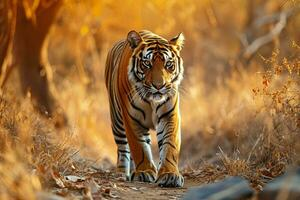
\includegraphics[width=0.2\textwidth]{figs/sample.jpg} \\
       % Department Name\\
       % University Name\\
       % Country\\
       তারিখঃ \today (১২ই ভাদ্র ১৩২১ বঙ্গাব্দ)
            
   \end{center}
\end{titlepage}
\tableofcontents
\newpage
\section{প্রথম অধ্যায়}
বাংলা ভাষা (বাঙলা, বাঙ্গলা, তথা বাঙ্গালা নামেও পরিচিত) একটি ধ্রুপদী ইন্দো-আর্য ভাষা, যা দক্ষিণ এশিয়ার বাঙালি জাতির প্রধান কথ্য ও লেখ্য ভাষা। মাতৃভাষীর সংখ্যায় বাংলা ইন্দো-ইউরোপীয় ভাষা পরিবারের পঞ্চম~\cite{reference1} ও মোট ব্যবহারকারীর~\cite{reference2} সংখ্যা অনুসারে বাংলা বিশ্বের ৭ম বৃহত্তম ভাষা, এবং দাপ্তরিক ভাষা হিসেবে বাংলা ভাষার অবস্থান ১০ম~\cite{ক০২}।

\subsection{প্রথম উপাধ্যায়}
বাংলা সার্বভৌম ভাষাভিত্তিক জাতিরাষ্ট্র বাংলাদেশের একমাত্র রাষ্ট্রভাষা তথা সরকারি ভাষা এবং ভারতের পশ্চিমবঙ্গ, ত্রিপুরা ও আসামের বরাক উপত্যকার দাপ্তরিক ভাষা। বঙ্গোপসাগরে অবস্থিত আন্দামান দ্বীপপুঞ্জের প্রধান কথ্য ভাষা বাংলা। এছাড়া, ভারতের ঝাড়খণ্ড, বিহার, মেঘালয়, মিজোরাম, ওড়িশার মতো রাজ্যগুলোতে উল্লেখযোগ্য পরিমাণে বাংলাভাষী জনগণ রয়েছে। 

\subsubsection{প্রথম উপ-উপাধ্যায়}
২০১১ সালের আদমশুমারি অনুযায়ী, ভারতের মোট জনসংখ্যার \textit{৮.০৩ শতাংশ} মানুষ বাংলা ভাষায় কথা বলে[১২] এবং হিন্দির পরেই বাংলা ভারতে সর্বাধিক প্রচলিত ভাষা। এছাড়াও মধ্যপ্রাচ্য, আমেরিকা ও ইউরোপে উল্লেখযোগ্য পরিমাণে বাংলাভাষী অভিবাসী রয়েছে সারা বিশ্বে সব মিলিয়ে \textbf{২৮.৫ কোটিরও} অধিক লোক দৈনন্দিন জীবনে বাংলা ব্যবহার করে।

\subsubsection{\englishfont In English}
{\englishfont 
Bengali, also known by its endonym Bangla, is a classical Indo-Aryan language from the Indo-European language family native to the Bengal region of South Asia. With over 237 million native speakers and another 41 million as second language speakers as of 2024, Bengali is the fifth most-spoken native language and the seventh most-spoken language by the total number of speakers in the world. It is the fifth most spoken Indo-European language~\cite{reference2}.

Adding new sentence for testing. 
}

\section{ইতিহাস}
বাংলা ভাষার ইতিহাসকে সাধারণত তিন ভাগে ভাগ করা হয়

\begin{enumerate}
    \item প্রাচীন বাংলা
    \item মধ্য বাংলা
    \item আধুনিক বাংলা
\end{enumerate}

বাংলায় প্রায় ৭৫,০০০ পৃথক শব্দ রয়েছে, যার মধ্যে

\begin{itemize}
    \item ৫০,২৫০ (৬৭\%) শব্দ "তৎসম" (সংস্কৃত ভাষা থেকে সরাসরি গৃহীত);
    \item ২১,০০০ (২৮\%) শব্দ "তদ্ভব" (বাংলা ভাষার শব্দসমূহ যার উৎস পালি এবং প্রাকৃত ভাষা থেকে হয়েছে);
    \item প্রায় ৫০০০ টি বিদেশি শব্দ
\end{itemize}
%%%%%%%%%%%%%%%%%%%%%%%%%%%%%%%%%%%%%%%%%%%%%%%%%%
%%% Bibliography %%%
\bibliographystyle{plain} 
\bibliography{reference.bib}
\end{document}
